\documentclass[11pt]{standalone}
\usepackage{amssymb}
\usepackage{amsmath}
\usepackage[no-math]{fontspec}
\usepackage{unicode-math}
\usepackage{libertinus}
\usepackage{pgf,xcolor}
\usepackage{tikz}
\usetikzlibrary{arrows.meta, backgrounds}
\usepackage{pgfplots}
\pgfplotsset{compat=newest}

\definecolor{my_darkgray}{HTML}{484949}
\definecolor{my_lightgray}{HTML}{F3F4F4}
\definecolor{my_darkblue}{HTML}{005A94}
\definecolor{my_lightblue}{HTML}{CCDEE9}
\definecolor{my_yellow}{HTML}{FFEC7F}
\definecolor{my_red}{HTML}{E60000}
\definecolor{my_orange}{HTML}{E87846}

\begin{document}
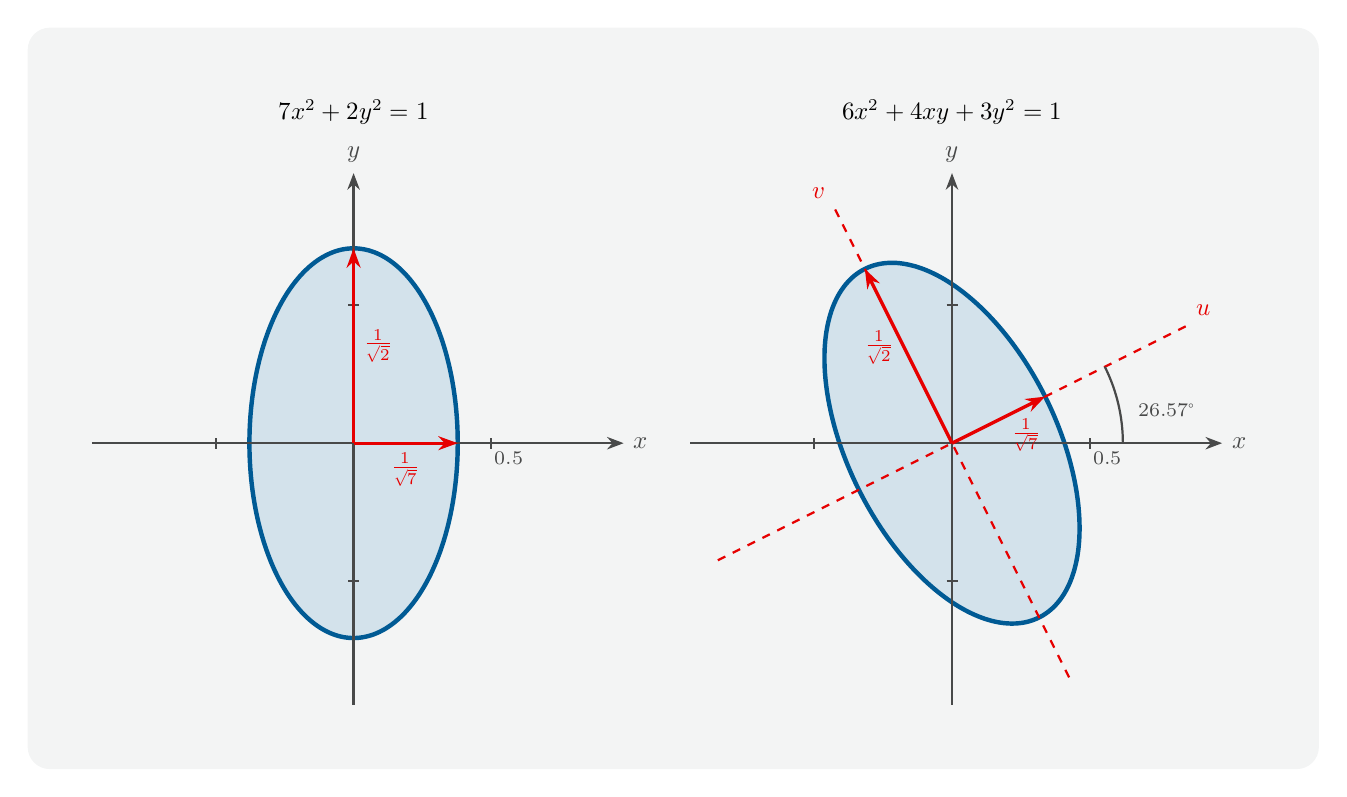
\begin{tikzpicture}[
    show background rectangle,
    background rectangle/.style={fill=my_lightgray, rounded corners=8pt},
    inner frame sep=0.8cm,
    x=3.5cm, y=3.5cm,
    vec/.style={-{Stealth[length=7pt, width=5pt]}, very thick}
]

% ---------------------------------------------------------------
%  Links:  x^T D x = 7x^2 + 2y^2 = 1,  D = diag(7, 2)
%          Halbachsen 1/sqrt(7) auf der x-Achse, 1/sqrt(2) auf der y-Achse
%  Rechts: x^T A x = 6x^2 + 4xy + 3y^2 = 1,  A = (6 2; 2 3)
%          dieselbe Ellipse, um 26.565 Grad gedreht (Q = R(26.565))
%          u-Achse in Richtung (2, 1), v-Achse in Richtung (-1, 2)
% ---------------------------------------------------------------

\newcommand{\achsen}{
    \draw[-{Stealth[length=6pt]}, thick, my_darkgray] (-0.95, 0) -- (0.98, 0)
        node[right, font=\small] {$x$};
    \draw[-{Stealth[length=6pt]}, thick, my_darkgray] (0, -0.95) -- (0, 0.98)
        node[above, font=\small] {$y$};
    \foreach \t in {-0.5, 0.5}{
        \draw[my_darkgray, thick] (\t, -0.02) -- (\t, 0.02);
        \draw[my_darkgray, thick] (-0.02, \t) -- (0.02, \t);
    }
    \node[below right, font=\scriptsize, my_darkgray, inner sep=1pt]
        at (0.5, -0.02) {$0.5$};
}

\newcommand{\ellipse}{
    \filldraw[fill=my_lightblue, fill opacity=0.8, draw=my_darkblue, ultra thick]
        plot[domain=0:360, samples=120, smooth cycle]
        ({cos(\x)/sqrt(7)}, {sin(\x)/sqrt(2)});
}

% ===== Linkes Teilbild: Ellipse in Hauptachsenlage =====
\begin{scope}
    \ellipse
    \achsen
    \draw[vec, my_red] (0, 0) -- ({1/sqrt(7)}, 0);
    \node[below, font=\small, my_red] at ({0.5/sqrt(7)}, 0)
        {$\frac{1}{\sqrt{7}}$};
    \draw[vec, my_red] (0, 0) -- (0, {1/sqrt(2)});
    \node[right, font=\small, my_red] at (0, {0.5/sqrt(2)})
        {$\frac{1}{\sqrt{2}}$};

    \node[font=\small] at (0, 1.2) {$7x^2 + 2y^2 = 1$};
\end{scope}

% ===== Rechtes Teilbild: gedrehte Ellipse mit Hauptachsen =====
\begin{scope}[xshift=7.6cm]
    \begin{scope}[rotate=26.565]
        \ellipse
    \end{scope}
    \achsen
    \begin{scope}[rotate=26.565]
        \draw[my_red, thick, dashed] (-0.95, 0) -- (0.95, 0)
            node[above right, font=\small, solid] {$u$};
        \draw[my_red, thick, dashed] (0, -0.95) -- (0, 0.95)
            node[above left, font=\small, solid] {$v$};
        \draw[vec, my_red] (0, 0) -- ({1/sqrt(7)}, 0);
        \node[below right, font=\small, my_red, inner sep=1pt]
            at ({0.6/sqrt(7)}, 0) {$\frac{1}{\sqrt{7}}$};
        \draw[vec, my_red] (0, 0) -- (0, {1/sqrt(2)});
        \node[left, font=\small, my_red] at (0, {0.55/sqrt(2)})
            {$\frac{1}{\sqrt{2}}$};
    \end{scope}
    \draw[my_darkgray, thick] (0.62, 0) arc[start angle=0, end angle=26.565,
        radius=0.62];
    \node[right, font=\scriptsize, my_darkgray] at (0.64, 0.12) {$26.57^\circ$};

    \node[font=\small] at (0, 1.2) {$6x^2 + 4xy + 3y^2 = 1$};
\end{scope}

\end{tikzpicture}
\end{document}
